%
% dual.tex -- Dualzahlen-Unterteilung
%
% (c) 2019 Prof Dr Andreas Müller, Hochschule Rapperswil
%
\documentclass[tikz]{standalone}
\usepackage{amsmath}
\usepackage{times}
\usepackage{txfonts}
\usepackage{pgfplots}
\usepackage{csvsimple}
\usetikzlibrary{arrows,intersections,math}
\begin{document}
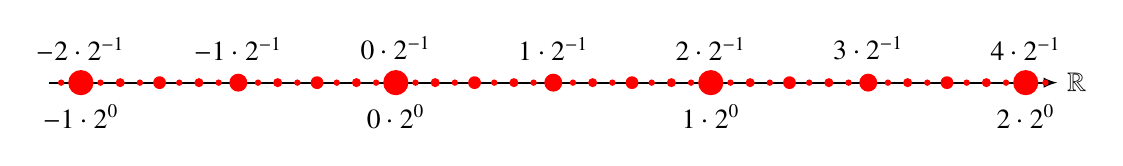
\begin{tikzpicture}[>=latex,scale=4]

\draw[->,line width=0.7pt]
	(-1.1,0)--(2.1,0) coordinate[label={right:$\mathbb R$}];

\def\s{0.04}


\foreach \x in {-1,...,2}{
	\node at ({\x},-\s) [below] {$\x\cdot 2^0$};
}

\foreach \x in {-2,...,4}{
	\node at ({\x/2},\s) [above] {$\x\cdot 2^{-1}$};
}

\foreach \x in {-1,...,2}{
	\fill[color=red] (\x,0) circle[radius=\s];
}

\def\f{1.4}

\pgfmathparse{\s/\f}
\xdef\s{\pgfmathresult}

\foreach \x in {-2,...,4}{
	\fill[color=red] ({\x/2},0) circle[radius={\s}];
}

\pgfmathparse{\s/\f}
\xdef\s{\pgfmathresult}

\foreach \x in {-4,...,8}{
	\fill[color=red] ({\x/4},0) circle[radius={\s}];
}

\pgfmathparse{\s/\f}
\xdef\s{\pgfmathresult}

\foreach \x in {-8,...,16}{
	\fill[color=red] ({\x/8},0) circle[radius=\s];
}

\pgfmathparse{\s/\f}
\xdef\s{\pgfmathresult}

\foreach \x in {-17,...,33}{
	\fill[color=red] ({\x/16},0) circle[radius=\s];
}


\end{tikzpicture}
\end{document}

